\documentclass{beamer}
\usepackage{tikz,amsmath,hyperref,graphicx,stackrel,animate}
\usetikzlibrary{positioning,shadows,arrows,shapes,calc}
\newcommand{\argmax}{\operatornamewithlimits{argmax}}
\newcommand{\argmin}{\operatornamewithlimits{argmin}}
\mode<presentation>{\usetheme{Frankfurt}}
\AtBeginSection[]
{
  \begin{frame}<beamer>
    \frametitle{Outline}
    \tableofcontents[currentsection,currentsubsection]
  \end{frame}
}
\title{Lecture 4: Filtered Noise}
\author{Mark Hasegawa-Johnson}
\date{ECE 417: Multimedia Signal Processing, Fall 2020}  
\begin{document}

% Title
\begin{frame}
  \maketitle
\end{frame}

% Title
\begin{frame}
  \tableofcontents
\end{frame}

%%%%%%%%%%%%%%%%%%%%%%%%%%%%%%%%%%%%%%%%%%%%
\section[Review]{Review: Power Spectrum}
\setcounter{subsection}{1}

\begin{frame}
  \frametitle{Review: Energy Spectrum and Parseval's Theorem}
  \begin{itemize}
  \item The energy spectrum of a random noise signal has the DTFT form
    $|X(\omega)|^2$, or the DFT form $|X[k]|^2$.
  \item The easiest form of Parseval's theorem to memorize is the DTFT
    energy spectrum form:
    \[
    \sum_{n=-\infty}^\infty x^2[n] = \frac{1}{2\pi}\int_{-\pi}^\pi |X(\omega)|^2d\omega
    \]
  \item The DFT energy spectrum form is similar, but over a finite duration:
    \[
    \sum_{n=0}^{N-1}x^2[n] = \frac{1}{N}\sum_{k=0}^{N-1}|X[k]|^2
    \]
  \end{itemize}
\end{frame}

\begin{frame}
  \frametitle{Review: Power Spectrum and Parseval's Theorem}
  Energy of an infinite-length signal might be infinite.  Wiener
  defined the {\bf power spectrum} in order to solve that problem:
  \[
  R_{xx}(\omega) = \lim_{N\rightarrow\infty} \frac{1}{N}|X(\omega)|^2
  \]
  where $X(\omega)$ is computed from a window of length $N$ samples.
  The DTFT power spectrum form of Parseval's theorem is
  \[
  \lim_{N\rightarrow\infty} \frac{1}{N}\sum_{n=-(N-1)/2}^{(N-1)/2}x^2[n] =
  \frac{1}{2\pi}\int_{-\pi}^\pi R_{xx}(\omega)d\omega
  \]
\end{frame}  

\begin{frame}
  \frametitle{White Noise}

  \begin{itemize}
    \item White noise is a type of noise whose samples are uncorrelated
      ($E[x[n]x[m]]=E[x[n]]E[x[m]]$, unless $n=m$).  If it is also zero mean
      and unit variance, then
      \begin{displaymath}
      E\left[x[n]x[m]\right] = \begin{cases}1 & n=m\\0&n\ne m\end{cases}
      \end{displaymath}
    \item The Fourier transform of any zero-mean random signal is,
      itself, a zero-mean random variable:
      \begin{displaymath}
        E\left[X(\omega)\right] = 0
      \end{displaymath}
    \item The power spectrum is also a random variable, but its
      expected value is not zero.  The expected power spectrum of
      white noise is flat, like white light:
      \begin{displaymath}
        E\left[R_{xx}(\omega)\right] =  E\left[\frac{1}{N}|X(\omega)|^2\right] = 1
      \end{displaymath}
  \end{itemize}
\end{frame}

\begin{frame}
  \frametitle{Example: DTFT and Power Spectrum of White Noise}
  
  \centerline{\includegraphics[height=2.5in]{exp/xpow.png}}
\end{frame}

\begin{frame}
  \frametitle{Example: Expected DTFT and  Power Spectrum of White Noise}
  
  \centerline{\includegraphics[height=2.5in]{exp/xexp.png}}
\end{frame}

\begin{frame}
  \frametitle{Colored Noise}

  \begin{itemize}
  \item Most colored noise signals are well modeled as filtered white
    noise, i.e., $y[n]=h[n]\ast x[n]$.  The filtering means that the
    samples of $y[n]$ are correlated with one another.
  \item If $x[n]$ is zero-mean, then so is $y[n]$, and so is $Y(\omega)$:
    \begin{displaymath}
      E\left[Y(\omega)\right] = 0
    \end{displaymath}
  \item The expected power spectrum is $|H(\omega)|^2$:
    \begin{displaymath}
      E\left[R_{yy}(\omega)\right] =  E\left[\frac{1}{N}|Y(\omega)|^2\right] = |H(\omega)|^2
    \end{displaymath}
  \end{itemize}
\end{frame}

\begin{frame}
  \frametitle{Example: Filtered Noise}
  
  \centerline{\includegraphics[height=2.5in]{exp/allspecs.png}}
\end{frame}

%%%%%%%%%%%%%%%%%%%%%%%%%%%%%%%%%%%%%%%%%%%%
\section[Autocorrelation]{Autocorrelation}
\setcounter{subsection}{1}

\begin{frame}
  \frametitle{Finite-Duration Power Spectrum}
  In practice, we will very often compute the power spectrum
  from a finite-length window:
  \[
  R_{xx}(\omega) = \frac{1}{N}|X(\omega)|^2,~~~R_{xx}[k]=\frac{1}{N}|X[k]|^2
  \]
  where $X(\omega)$ is computed from a window of length $N$ samples.
  The DTFT power spectrum form of Parseval's theorem is then
  \[
  \frac{1}{N}\sum_{n=0}^{N-1}x^2[n] =
  \frac{1}{2\pi}\int_{-\pi}^\pi R_{xx}(\omega)d\omega = \frac{1}{N}\sum_{k=0}^N R_{xx}[k]
  \]
\end{frame}

\begin{frame}
  \frametitle{Inverse DTFT of the Power Spectrum}

  Since the power spectrum of noise is MUCH more useful than the
  expected Fourier transform, let's see what the inverse Fourier transform of the power spectrum
  is.  Let's call $R_{xx}(\omega)$ the power spectrum, and $r_{xx}[n]$ its inverse
  DTFT.
  \[
  R_{xx}(\omega) = \frac{1}{N}|X(\omega)|^2 = \frac{1}{N}X(\omega)X^*(\omega)
  \]
  where $X^*(\omega)$ means complex conjugate.  Since multiplying the DTFT
  means convolution in the time domain, we know that
  \[
  r_{xx}[n] = \frac{1}{N} x[n]\ast z[n]
  \]
  where $z[n]$ is the inverse transform of $X^*(\omega)$ (we haven't
  figured out what that is, yet).
\end{frame}

\begin{frame}
  \frametitle{Inverse DTFT of the Power Spectrum}

  So what's the inverse DFT of $X^*(\omega)$?  If we assume that $x[n]$ is
  real, we get that
  \begin{align*}
    X^*(\omega) &= \left(\sum_{n=-\infty}^{\infty}x[n]e^{-j\omega n}\right)^*\\
    &= \sum_{n=-\infty}^{\infty}x[n]e^{j\omega n}\\
    &= \sum_{m=-\infty}^{\infty}x[-m]e^{-j\omega m}
  \end{align*}
  So if $x[n]$ is real, then the inverse DTFT of $X^*(\omega)$ is $x[-n]$!
\end{frame}
\begin{frame}
  \frametitle{Autocorrelation}
  The power spectrum, of an $N$-sample finite-length signal, is
  \[
  R_{xx}(\omega)=\frac{1}{N}|X(\omega)|^2
  \]
  Its inverse Fourier transform is the autocorrelation,
  \[
  r_{xx}[n] = \frac{1}{N}x[n]\ast x[-n]  = \frac{1}{N}\sum_{m=-\infty}^\infty  x[m] x[m-n]
  \]
  This relationship, $r_{xx}[n]\leftrightarrow R_{xx}(\omega)$, is called
  Wiener's theorem, named after Norbert Wiener, the inventor of
  cybernetics.
\end{frame}

\begin{frame}
  \frametitle{Example: Autocorrelation of White Noise}
  
  \centerline{\animategraphics[loop,controls,height=2.5in]{10}{exp/xcor}{1}{62}}
\end{frame}

\begin{frame}
  \frametitle{A warning about python}

  Notice, on the last slide, I defined autocorrelation as
  \[
  r_{xx}[n] = \frac{1}{N}x[n]\ast x[-n]  = \frac{1}{N}\sum_{m=-\infty}^\infty  x[m] x[m-n]
  \]
  Python defines an ``energy version'' of autocorrelation, instead of
  the ``power version'' shown above, i.e., {\tt np.correlate} computes:
  \[
  r_{\mbox{python}}[n] = \sum_{m=-\infty}^\infty x[m]x[m-n]
  \]
  The difference is just a constant factor ($N$), so it usually isn't
  important.  But sometimes you'll need to be aware of it.
\end{frame}
  
%\begin{frame}
%  \frametitle{Convolution vs. Autocorrelation}
%  \centerline{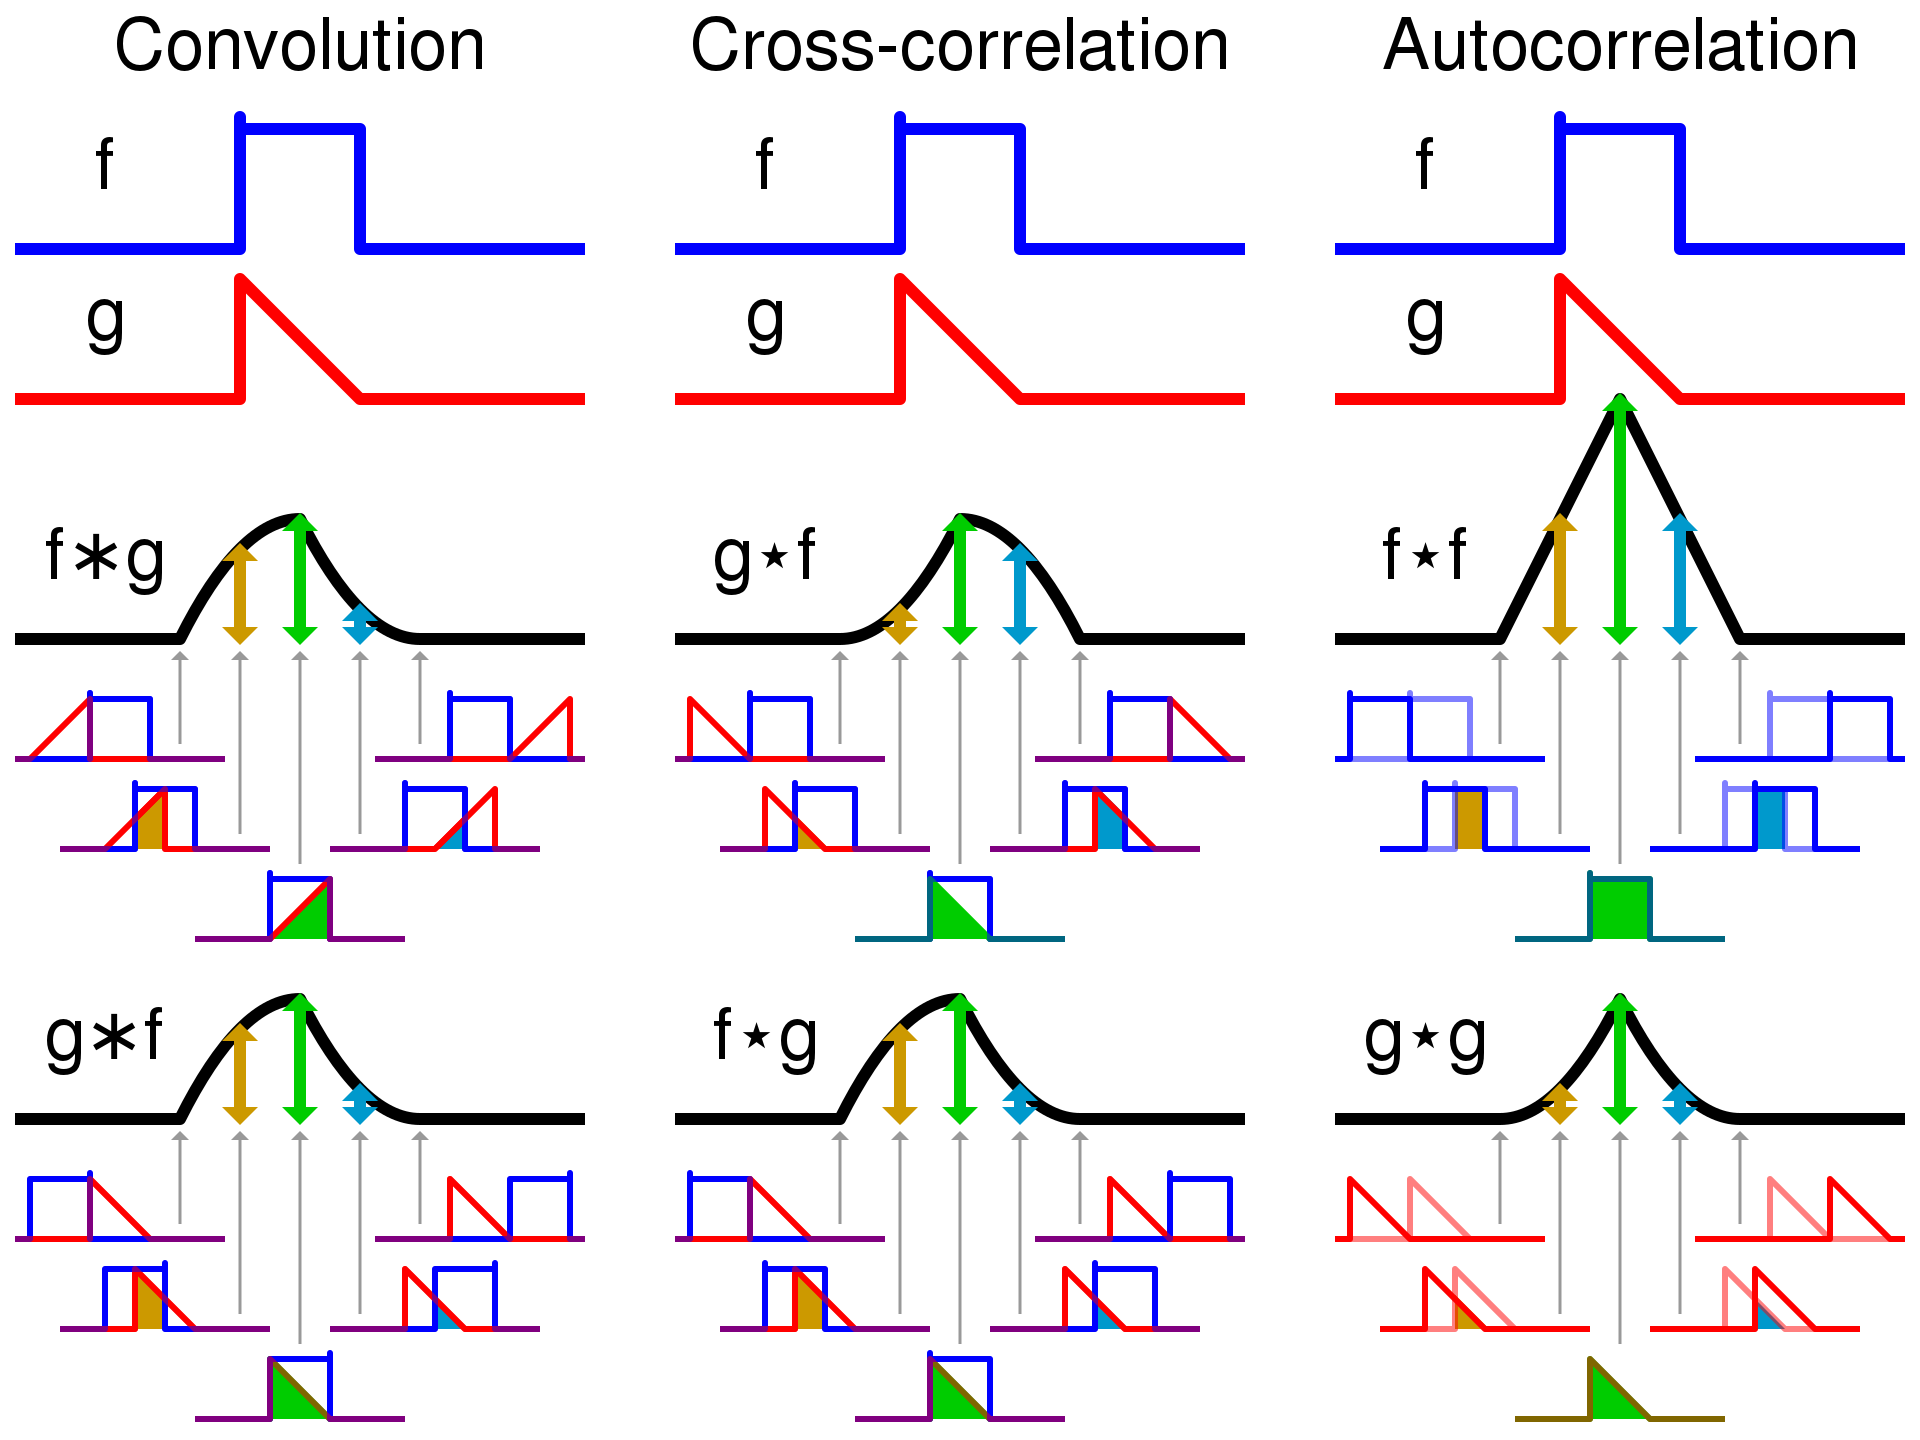
\includegraphics[height=2.5in]{Comparison_convolution_correlation.png}}
%  \begin{tiny}
%    By Cmglee, CC-SA 3.0,
%    \url{https://commons.wikimedia.org/wiki/File:Comparison_convolution_correlation.svg}
%  \end{tiny}
%\end{frame}

\begin{frame}
  \frametitle{Autocorrelation is also a random variable!}

  \begin{itemize}
    \item Notice that, just as the power spectrum is a random
      variable, the autocorrelation is also a random variable.
    \item The autocorrelation is the average of $N$ consecutive
      products, thus
      \[
      E\left[r_{xx}[n]\right] =
      E\left[\frac{1}{N}\sum_{m=0}^{N-1} x[m]x[m-n]\right]
      = E\left[x[m]x[m-n]\right]
      \]
    \item
      The expected autocorrelation is related to the covariance
      and the mean:
      \[
      E\left[r_{xx}[n]\right] =\mbox{Cov}\left(x[m],x[m-n]\right)+E\left[x[m]\right]E\left[x[m-n]\right]
      \]
    \item
      If $x[n]$ is zero-mean, that means
      \[
      E\left[r[n]\right] =\mbox{Cov}\left(x[m],x[m-n]\right)
      \]
  \end{itemize}
\end{frame}
\begin{frame}
  \frametitle{Autocorrelation of white noise}
  If $x[n]$ is zero-mean white noise, with a variance of $\sigma^2$, then
  \[
  E\left[r_{xx}[n]\right] =
  E\left[x[m]x[m-n]\right]= \begin{cases} \sigma^2 & n=0\\0 &\mbox{otherwise}\end{cases}
  \]
  We can write
  \[
  E\left[r[n]\right]=\sigma^2\delta[n]
  \]
\end{frame}

%%%%%%%%%%%%%%%%%%%%%%%%%%%%%%%%%%%%%%%%%%%%
\section[Autocorrelation]{Autocorrelation of Filtered Noise}
\setcounter{subsection}{1}

\begin{frame}
  \frametitle{Filtered Noise}

  What happens when we filter noise?  Suppose that $x[n]$ is zero-mean
  white noise, and
  \[
  y[n] = h[n]\ast x[n]
  \]
  What is $y[n]$?
\end{frame}

\begin{frame}
  \frametitle{Example: Filtering of White Noise}
  
  \centerline{\animategraphics[loop,controls,height=2.5in]{10}{exp/xhy}{0}{63}}
\end{frame}

\begin{frame}
  \frametitle{Filtered Noise}
  \[
  y[n] = h[n]\ast x[n] = \sum_{m=-\infty}^\infty h[m]x[n-m]
  \]
  \begin{itemize}
  \item $y[n]$ is the sum of zero-mean random variables, so it's also
    zero-mean.
  \item $y[n]=h[0]x[n]+\mbox{other stuff}$, and
    $y[n+1]=h[1]x[n]+\mbox{other stuff}$.  So obviously, $y[n]$ and
    $y[n+1]$ are not uncorrelated.  So $y[n]$ is not white noise.
  \item What kind of noise is it?
  \end{itemize}
\end{frame}

\begin{frame}
  \frametitle{The variance of $y[n]$}

  First, let's find its variance.  Since $x[n]$ and $x[n+1]$ are
  uncorrelated, we can write
  \begin{align*}
    \sigma_y^2 &= \sum_{m=-\infty}^\infty h^2[m] \mbox{Var}(x[n-m])\\
    &= \sigma_x^2 \sum_{m=-\infty}^\infty h^2[m]
  \end{align*}
\end{frame}

\begin{frame}
  \frametitle{The autocorrelation of $y[n]$}

  Second, let's find its autocorrelation.  Let's define $r_{xx}[n] = \frac{1}{N} x[n]\ast x[-n]$.
  Then
  \begin{align*}
    r_{yy}[n] &= \frac{1}{N} y[n] \ast y[-n]\\
    &= \frac{1}{N} (x[n]\ast h[n]) \ast (x[-n]\ast h[-n])\\
    &= \frac{1}{N} x[n]\ast x[-n]\ast h[n]\ast h[-n]\\
    &= r_{xx}[n] \ast h[n]\ast h[-n]
  \end{align*}
\end{frame}

\begin{frame}
  \frametitle{Example: Autocorrelation of Colored Noise}
  
  \centerline{\animategraphics[loop,controls,height=2.5in]{10}{exp/ycor}{1}{62}}
\end{frame}

\begin{frame}
  \frametitle{Expected autocorrelation of $y[n]$}

  \[
  r_{yy}[n] = r_{xx}[n] \ast h[n]\ast h[-n]
  \]
  Expectation is linear, and convolution is linear, so
  \[
  E\left[r_{yy}[n]\right] = E\left[r_{xx}[n]\right] \ast h[n]\ast h[-n]
  \]
\end{frame}

\begin{frame}
  \frametitle{Expected autocorrelation of $y[n]$}
  
  $x[n]$ is zero-mean white noise if and  only if its autocorrelation is a delta function:
  \[
  E\left[r_{xx}[n]\right] = \sigma_x^2 \delta[n]
  \]
  If $y[n]=h[n]\ast x[n]$, and $x[n]$ is zero-mean white noise, then
  \[
  E\left[r_{yy}[n]\right] = \sigma_x^2 \left(h[n]\ast h[-n]\right)
  \]
  In other words, $x[n]$ contributes only its energy ($\sigma_x^2$).  $h[n]$ contributes the
  correlation between neighboring  samples.
\end{frame}

\begin{frame}
  \frametitle{Example: Expected Autocorrelation of Colored Noise}
  
  \centerline{\animategraphics[loop,controls,height=2.5in]{10}{exp/hcor}{1}{62}}
\end{frame}

\begin{frame}
  \frametitle{Example}

  Here's an example.  The white noise signal on the top ($x[n]$) is
  convolved with the bandpass filter in the middle ($h[n]$) to produce
  the green-noise signal on the bottom ($y[n]$).  Notice that $y[n]$
  is random, but correlated.
  
  \centerline{\includegraphics[height=2in]{../lec18/exp/gtfiltered_white_waveform.png}}
\end{frame}

\begin{frame}
  \frametitle{Example}

  Here's another example.  The white noise signal on the left ($x[n]$) is
  convolved with an ideal lowpass filter, with a cutoff at $\pi/2$, to create 
  the pink-noise signal on the right ($y[n]$).  Notice that $y[n]$
  is random, but correlated.
  
  \centerline{\includegraphics[width=2in]{../lec18/exp/whitefreqandtime.png}
    \includegraphics[height=2in]{../lec18/exp/pinkfreqandtime.png}}
\end{frame}

\begin{frame}
  \frametitle{Example}

  Here's a third example.  The white noise signal on the left ($x[n]$)
  is convolved with an ideal highpass filter, with a cutoff at
  $\pi/2$, to create the blue-noise signal on the right ($y[n]$).
  Here, it's a lot less obvious that the samples of $y[n]$ are
  correlated with one another, but they are: in fact, they are {\bf
    negatively correlated}.  If $y[n]>0$, then $y[n+1]<0$ with a
  probability greater than 50\%.
  
  \centerline{\includegraphics[width=2in]{../lec18/exp/whitefreqandtime.png}
    \includegraphics[height=2in]{../lec18/exp/bluefreqandtime.png}}
\end{frame}

%%%%%%%%%%%%%%%%%%%%%%%%%%%%%%%%%%%%%%%%%%%%
\section[Spectrum]{Power Spectrum of Filtered Noise}
\setcounter{subsection}{1}

\begin{frame}
  \frametitle{Power Spectrum of Filtered Noise}

  So we have $r_{yy}[n]=r_{xx}[n]\ast h[n]\ast h[-n]$.  What about the
  power spectrum?

  \begin{align*}
    R_{yy}(\omega) &= {\mathcal F}\left\{r_{yy}[n]\right\} \\
    &= {\mathcal F}\left\{r_{xx}[n]\ast h[n]\ast h[-n]\right\} \\
    &= R_{xx}(\omega)|H(\omega)|^2
  \end{align*}
\end{frame}

\begin{frame}
  \frametitle{Example}

  Here's an example.  The white noise signal on the top ($|X[k]|^2$)
  is multiplied by the bandpass filter in the middle ($|H[k]|^2$) to
  produce the green-noise signal on the bottom
  ($|Y[k]|^2=|X[k]|^2|H[k]|^2$).
  
  \centerline{\includegraphics[height=2in]{../lec18/exp/gtfiltered_white_powerspectrum.png}}
\end{frame}

\begin{frame}
  \frametitle{Units Conversion}

  The DTFT version of Parseval's theorem, assuming a finite window of
  length $N$ samples, is
  \[
  \frac{1}{N}\sum_{n} x^2[n] = \frac{1}{2\pi}\int_{-\pi}^{\pi} R_{xx}(\omega)d\omega
  \]
  Let's consider converting units to Hertz.  Remember that
  $\omega=\frac{2\pi f}{F_s}$, where $F_s$ is the sampling frequency, so
  $d\omega = \frac{2\pi}{F_s}df$, and we get that
  \[
  \frac{1}{N}\sum_{n} x^2[n] = \frac{1}{F_s}\int_{-F_s/2}^{F_s/2} R_{xx}\left(\frac{2\pi f}{F_s}\right)df
  \]
  So we can use $R_{xx}\left(\frac{2\pi f}{F_s}\right)$ as if it were
  a power spectrum in continuous time, at least for
  $-\frac{F_s}{2}<f<\frac{F_s}{2}$.
\end{frame}

\begin{frame}
  \frametitle{Example: Power Spectrum of Colored Noise}
  
  \centerline{\includegraphics[height=2.5in]{exp/ypow.png}}
\end{frame}

\begin{frame}
  \frametitle{Example: Expected Power Spectrum of Colored Noise}
  
  \centerline{\includegraphics[height=2.5in]{exp/yexp.png}}
\end{frame}

%%%%%%%%%%%%%%%%%%%%%%%%%%%%%%%%%%%%%%%%%%%%
\section[Parseval]{Parseval's Theorem}
\setcounter{subsection}{1}

\begin{frame}
  \frametitle{Parseval's Theorem}

  Now we have everything we need to prove Parseval's theorem.  Let's
  prove the DTFT power form of the theorem, for a finite-length
  signal:
  \begin{displaymath}
    \frac{1}{N}\sum_{n=0}^{N-1} x^2[n] = \frac{1}{2\pi}\int_{-\pi}^\pi R_{xx}(\omega)  d\omega
  \end{displaymath}
  where
  \begin{displaymath}
    R_{xx}(\omega) = \frac{1}{N}|X(\omega)|^2
  \end{displaymath}
\end{frame}

\begin{frame}
  \frametitle{Parseval's Theorem}

  \begin{displaymath}
    \frac{1}{N}\sum_{n=0}^{N-1} x^2[n] = \frac{1}{2\pi}\int_{-\pi}^\pi R_{xx}(\omega)  d\omega
  \end{displaymath}
  Notice that the left-hand side is the autocorrelation, with a lag of $0$:
  \begin{displaymath}
    r_{xx}[m] = \frac{1}{N}\sum_{n=0}^{N-1} x[n]x[n-m]
  \end{displaymath}
  So Parseval's theorem is just  saying that
  \begin{displaymath}
    r_{xx}[0] = \frac{1}{2\pi}\int_{-\pi}^\pi R_{xx}(\omega)  d\omega
  \end{displaymath}
\end{frame}

\begin{frame}
  \frametitle{Wiener's Theorem}

  Wiener's theorem says that the power spectrum is the Fourier
  transform of the autocorrelation:
  \begin{displaymath}
    r_{xx}[n] = \frac{1}{2\pi}\int_{-\pi}^\pi R_{xx}(\omega)e^{j\omega n}d\omega
  \end{displaymath}
  But notice what happens if we plug in $n=0$:
  \begin{displaymath}
    r_{xx}[0] = \frac{1}{2\pi}\int_{-\pi}^\pi R_{xx}(\omega)d\omega
  \end{displaymath}
  Q.E.D.
\end{frame}

%%%%%%%%%%%%%%%%%%%%%%%%%%%%%%%%%%%%%%%%%%%%
\section[Example]{Example}
\setcounter{subsection}{1}

\begin{frame}
  \frametitle{Example: Autocorrelation of White Noise}
  
  \centerline{\animategraphics[loop,controls,height=2.5in]{10}{exp/xcor}{1}{62}}
\end{frame}

\begin{frame}
  \frametitle{Example: Power Spectrum of White Noise}
  
  \centerline{\includegraphics[height=2.5in]{exp/xpow.png}}
\end{frame}

\begin{frame}
  \frametitle{Example: Expected Power Spectrum of White Noise}
  
  \centerline{\includegraphics[height=2.5in]{exp/xexp.png}}
\end{frame}

\begin{frame}
  \frametitle{Example: Filtering of White Noise}
  
  \centerline{\animategraphics[loop,controls,height=2.5in]{10}{exp/xhy}{0}{63}}
\end{frame}

\begin{frame}
  \frametitle{Example: Power Spectra of White and Colored Noises}
  
  \centerline{\includegraphics[height=2.5in]{exp/allspecs.png}}
\end{frame}

\begin{frame}
  \frametitle{Example: Autocorrelation of Colored Noise}
  
  \centerline{\animategraphics[loop,controls,height=2.5in]{10}{exp/ycor}{1}{62}}
\end{frame}

\begin{frame}
  \frametitle{Example: Power Spectrum of Colored Noise}
  
  \centerline{\includegraphics[height=2.5in]{exp/ypow.png}}
\end{frame}

\begin{frame}
  \frametitle{Example: Expected Power Spectrum of Colored Noise}
  
  \centerline{\includegraphics[height=2.5in]{exp/yexp.png}}
\end{frame}


%%%%%%%%%%%%%%%%%%%%%%%%%%%%%%%%%%%%%%%%%%%%
\section[Summary]{Summary}
\setcounter{subsection}{1}

\begin{frame}
  \frametitle{Wiener's Theorem and Parseval's Theorem}
  \begin{itemize}
  \item Wiener's theorem says that the power spectrum is the DTFT of
    autocorrelation:
    \begin{displaymath}
      r_{xx}[n] = \frac{1}{2\pi}\int_{-\pi}^\pi R_{xx}(\omega)e^{j\omega n}d\omega
    \end{displaymath}
  \item Parseval's theorem says that average power in the time domain
    is the same as average power in the frequeny domain:
    \begin{displaymath}
      r_{xx}[0] = \frac{1}{2\pi}\int_{-\pi}^\pi R_{xx}(\omega)d\omega
    \end{displaymath}
  \end{itemize}
\end{frame}

\begin{frame}
  \frametitle{Filtered Noise}

  If $y[n]=h[n]\ast x[n]$, $x[n]$ is any noise signal, then
  \begin{align*}
    r_{yy}[n] &= r_{xx}[n]\ast h[n]\ast h[-n]\\
    R_{yy}(\omega) &= R_{xx}(\omega) |H(\omega)|^2
  \end{align*}
\end{frame}
  
\begin{frame}
  \frametitle{White Noise and Colored Noise}
  
  If $x[n]$ is zero-mean unit variance white noise, and $y[n]=h[n]\ast
  x[n]$, then
  \begin{align*}
    E\left[r_{xx}[n]\right] &= \delta[n]\\
    E\left[R_{xx}(\omega)\right] &= 1\\
    E\left[r_{yy}[n]\right] &= h[n]\ast h[-n]\\
    E\left[R_{yy}(\omega)\right] &= |H(\omega)|^2
  \end{align*}
\end{frame}

\end{document}
